\documentclass{chi2009}
\usepackage{times}
\usepackage{url}
\usepackage{graphics}
\usepackage{color}
\usepackage[pdftex]{hyperref}
\hypersetup{%
pdftitle={TwinList: \\ \large Visualizing List Differences},
pdfauthor={Leonardo Max Baptista Claudino, claudino@cs.umd.edu \\
	    Sameh Khamis, sameh@cs.umd.edu \\
	    Ran Liu, ranliu@cs.umd.edu \\
	    Ben London, blondon@cs.umd.edu \\
	    Jay Pujara, jay@cs.umd.edu},
pdfkeywords={list visualization},
bookmarksnumbered,
pdfstartview={FitH},
colorlinks,
citecolor=black,
filecolor=black,
linkcolor=black,
urlcolor=black,
breaklinks=true,
}
\newcommand{\comment}[1]{}
\definecolor{Orange}{rgb}{1,0.5,0}
\newcommand{\todo}[1]{\textsf{\textbf{\textcolor{Orange}{[[#1]]}}}}

\pagenumbering{arabic}  % Arabic page numbers for submission.  Remove this line to eliminate page numbers for the camera ready copy

\begin{document}
% to make various LaTeX processors do the right thing with page size
\special{papersize=8.5in,11in}
\setlength{\paperheight}{11in}
\setlength{\paperwidth}{8.5in}
\setlength{\pdfpageheight}{\paperheight}
\setlength{\pdfpagewidth}{\paperwidth}

% use this command to override the default ACM copyright statement 
% (e.g. for preprints). Remove for camera ready copy.
\toappear{Submitted for CMSC 734 Information Visualization.}

\title{TwinList: \\ \large Visualizing List Differences}
\numberofauthors{5}
\author{
  \alignauthor Leonardo Max Batista Claudino \\
    \affaddr{Dept. of Computer Science, University of Maryland}\\
    \affaddr{College Park, MD 20742}\\
    \email{claudino@cs.umd.edu}
  \and
  \alignauthor Sameh Khamis\\
    \affaddr{Dept. of Computer Science, University of Maryland}\\
    \affaddr{College Park, MD 20742}\\
    \email{sameh@cs.umd.edu}
  \and
  \alignauthor Ran Liu \\
    \affaddr{Dept. of Computer Science, University of Maryland}\\
    \affaddr{College Park, MD 20742}\\
    \email{ranliu@cs.umd.edu}
  \and
  \alignauthor Ben London \\
    \affaddr{Dept. of Computer Science, University of Maryland}\\
    \affaddr{College Park, MD 20742}\\
    \email{blondon@cs.umd.edu}
  \and
  \alignauthor Jay Pujara \\
    \affaddr{Dept. of Computer Science, University of Maryland}\\
    \affaddr{College Park, MD 20742}\\
    \email{jay@cs.umd.edu}
}

\maketitle

\begin{abstract}
We present a novel list visualization tool named TwinList, for the purpose of list visualization and matching. Leveraging Adobe's Flex platform and the Prefuse Flare toolbox, we created a rich internet application (RIA) with dynamic animated effects. These animated transitions lead the user through the procedure of matching two lists, using color coding to highlight the similarities and differences between the two. List items can be grouped, sorted and filtered according to their attribute values, to enhance workflow. To illustrate the efficacy of the application, we conduct usability testing with several doctors and peers.
\end{abstract}

\keywords{list visualization} 

\category{H.5.2}{Information Interfaces and Presentation}{Miscellaneous}[Optional sub-category]

\section{Introduction}
In applications involving list-based data, it is often necessary to match similar items and take some action on the list elements. One such domain is that of medical list reconciliation, in which a physician must reconcile a patient's medication from multiple prescribers.
\subsection{Related Work}

\section{TwinList}
TwinList is a novel list visualization tool, with the purpose of showing the similarity and difference of two lists. It can be used in many cases where the comparison of two lists of items is required. The major task that TwinList support is medication reconciliation, comparing a patient's medication orders to all of the medications that a patient has been taking\cite{JCAHO-2006}.  However, the application for Twinlist is not only for medication reconciliation, but also for general list data, for example, comparing two lists of words used in the State of The Union speech by Bush and Obama. 

TwinList interface consists four major components: the list viewer, controlling panel, accept/reject list and detail panel, as shown in (Figure~\ref{interface}).


\begin{figure}
\begin{center}
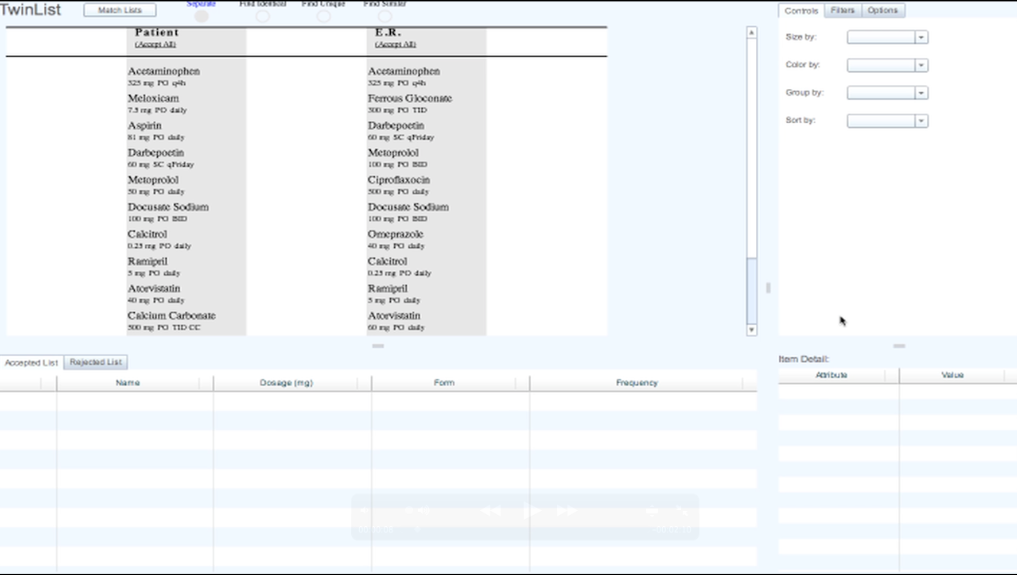
\includegraphics[width=1.1\linewidth]{interface}
\end{center}
   \caption{TwinList interface}
   \label{interface}
\end{figure}


\subsection{ListViewer}

\subsection{Controls}

\subsection{Filters}

\subsection{Options}

\section{Evaluation}

We are currently working on a prototype of our visualization, thus we are more concerned with qualitative than quantitative feedback about the features of our visualization system at this point. That way, according to the categorization proposed by Lam et al~\cite{lam-bertini-isenberg-plaisant-carpendale-2011}, the evaluation scenario best matching our present purposes is the \textit{User Experience (UE)} test case. The goal of the experiments we propose in this study was to observe how users react to the visualization and interaction features offered by TwinList. We will use the provided feedback to improve the system's design in future versions. 

\subsection{Experiment Design}

Our test subjects came two specific populations: 2 physicians that used the system to perform medication reconciliation and 2 general public participants that used TwinList to operate on State of Union speech lists to look for insightful patterns. In short, the testing protocol basically consisted of the following: first, the user watched a $~7$-minutes video with basic usage demonstration.  Then, they were allowed to ask questions. Next, users interacted with the system and either performed specific tasks (medication reconciliation case studies) or freely used the system trying to look for interesting patterns (State of the Union speech experiments). While using the system, subjects were encouraged to \textit{think aloud} and both the video and audio were recorded. 

\subsection{Case 1: Med. reconciliation, A. Z. H., male, 34 y. o.}

Overall, the user performed the tasks as expected and reported correct results. A. Z. H. reported to be very confortable with computers. He does not do medication reconciliation on a regular basis, but when doing inpatient aid and discharge from hospital, for which he does not use any software. This is how he describes his TwinList experience: \textit{"It's really impressive, the way you organize things is great. It's definitely a step in the right direction ..."}. This particular subject was very keen on doing the test and came up with several suggestions, most of all worth including in this section. 

\subsubsection{Results}
This is our reading of A. Z. H. experience:
\begin{itemize}
\item There is need for an indication that there are more items than what can be currently seen in a column. Only the scroll bar would not be sufficient.
\item It is hard to getting to the \textit{Accept/Reject} pop-up menu when accepting/rejecting an item. He had trouble to click and hold, and even tried to right-click to get to the menu.
\item To send items from \textit{Accept/Reject} lists back to the viewer one-by-one requires quite some effort when you have several items in those lists. A \textit{Remove All} button would be desirable.
\item Warning dialogs or undo may be needed when accepting and rejecting items, since it is a delicate operation in medication reconciliation.
\item In the control panel, drop-down boxes should have what the default \textit{Group by}/\textit{Sort by} are, instead of blank captions.
\item It would be desirable to shorten vertical empty spaces in between items to minimize the need of scrolling.
\item We should reduce the number of visible attributes of an item in the \textit{List View}, since reconciliation is done, in practice, based on only a few of them (e. g. the \textit{Indication} feature).
\item For items in the \textit{Similar} columns, the item pop-up menu should have a third option that would be to automatically reject an item of a list if its counterpart at the other list was accepted. According to the participant, this will be the case almost every time items are accepted/rejected.
\item He suggested that we should change the way items are displayed so that, for each list, you have items sorted by its \textit{uniqueness level}, for example, by vertically ranging from identical to unique. That would add more meaning to the vertical structure of the list, which is somewhat lost after lists are matched, but would represent a significant change in the concept.
\item The user feels that the \textit{Accepted/Rejected} lists down at the bottom may not be sufficient to track what happened to processed items in the lists, especially if he gets distracted. He also missed being able to interact on the spot with accepted/rejected items that are grayed out. In his words: \textit{"If it is grayed out, what if (...) I really wanna do the 100 mg, is there any way to click and have it re-instate (...) or un-reject/un-accept"}. He thinks that if he could interact with grayed-out items on the viewer, the \textit{Accepted/Rejected} lists might not even be needed, therefore allowing more room to the main viewer panel. Along that line, the list of rejected/accepted items would come out as a final product of the interactive process and would be activated by pressing a button, as he mentioned: \textit{"... Here is your final list of medications, this is your rejected list over here, and when one finally accepts, export to (...) or put in patient's medical record ..."}.
\item He also suggested a sort by, in his own words, \textit{"medications that haven't been dealt yet"} which we would translate into grouping medications based on whether they have been accepted/rejected or not, in fact a nice general concept applicable to other list matching problems.
\item The user mentioned the importance of filters, especially to filter by route (e. g. I.V. medications).  
\end{itemize}

\section{Conclusion}

\bibliographystyle{abbrv}
\bibliography{twinlist}

\end{document}
